\subsection{Development process}

	\subsubsection{Agile model}
	
	Agile software development uses iterative development as a basis but advocates a lighter and more people-centric viewpoint than traditional approaches. Agile processes use feedback, rather than planning, as their primary control mechanism. The feedback is driven by regular tests and releases of the evolving software. \cite{wiki:development-process}
	
	The most used agile model for iterative, incremental framework this days is SCRUM. Although the Scrum approach was originally suggested for managing product development projects, its use has focused on the management of software development projects, and it can be used to run software maintenance teams or as a general project/program management approach.\newline
	
	Scrum is a process skeleton that contains sets of practices and predefined roles. The main roles in Scrum are:
	
	\begin{itemize}
		\item the “ScrumMaster”, who maintains the processes (typically in lieu of a project manager)
		\item the “Product Owner”, who represents the stakeholders and the business
		\item the “Team”, a cross-functional group who do the actual analysis, design, implementation, testing, etc.
	\end{itemize}
	
	\begin{figure}[htb]
		\centering
		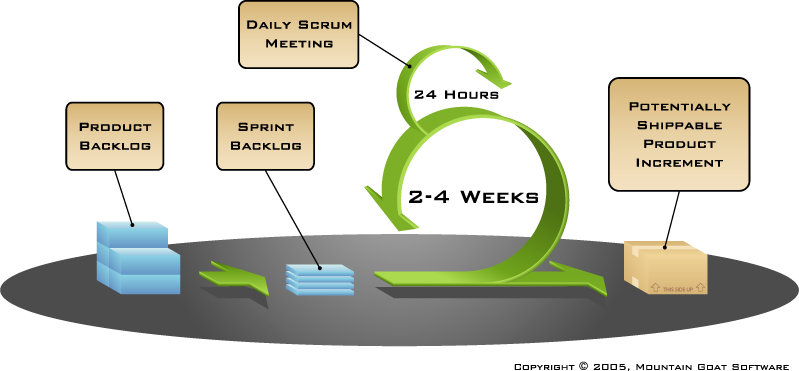
\includegraphics[width=0.8\textwidth]{prestudy/development_process/scrum.png}
		\caption{Scrum methodology}
		\label{fig:scrum-methology}
	\end{figure}
	
	During each “sprint”, typically a two to four week period (with the length being decided by the team), the team creates a potentially deliverable product increment (for example, working and tested software). The set of features that go into a sprint come from the product “backlog”, which is a prioritized set of high level requirements of work to be done. Which backlog items go into the sprint is determined during the sprint planning meeting. During this meeting, the Product Owner informs the team of the items in the product backlog that he or she wants completed. The team then determines how much of this they can commit to complete during the next sprint, and records this in the sprint backlog. During a sprint, no one is allowed to change the sprint backlog, which means that the requirements are frozen for that sprint. Development is timeboxed such that the sprint must end on time; if requirements are not completed for any reason they are left out and returned to the product backlog. After a sprint is completed, the team demonstrates how to use the software.\newline
	
	Scrum enables the creation of self-organizing teams by encouraging co-location of all team members, and verbal communication between all team members and disciplines in the project.\newline
	
	A key principle of Scrum is its recognition that during a project the customers can change their minds about what they want and need (often called requirements churn), and that unpredicted challenges cannot be easily addressed in a traditional predictive or planned manner. As such, Scrum adopts an empirical approach—accepting that the problem cannot be fully understood or defined, focusing instead on maximizing the team’s ability to deliver quickly and respond to emerging requirements.\newline

	\subsubsection{Waterfall model}
	The waterfall model is a sequential design process, often used in software development processes, in which progress is seen as flowing steadily downwards (like a waterfall) through the phases of Conception, Initiation, Analysis, Design, Construction, Testing, Production/Implementation and Maintenance.\newline
	
	\begin{figure}[htb]
		\centering
		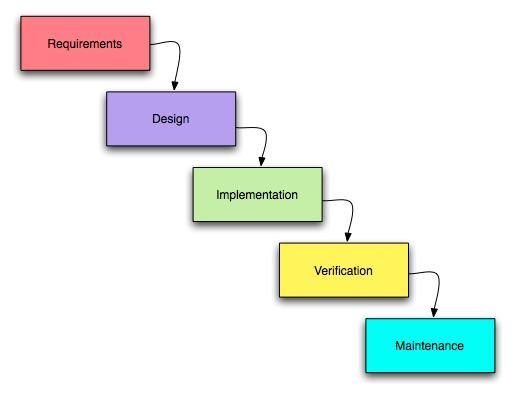
\includegraphics[width=0.8\textwidth]{prestudy/development_process/waterfall.jpg}
		\caption{The unmodified "waterfall model" methodology}
		\label{fig:waterfall-model}
	\end{figure}
	
	In Royce's original waterfall model, the following phases are followed in order:
	
	\begin{itemize}
		\item Requirements specification
		\item Design
		\item Construction (AKA implementation or coding) testing, etc.
		\item Integration
		\item Testing and debugging (AKA Validation)
		\item Installation
		\item Maintenance
	\end{itemize}
	
	Thus the waterfall model maintains that one should move to a phase only when its preceding phase is completed and perfected. However, there are various modified waterfall models (including Royce's final model) that may include slight or major variations upon this process.
